%%%%%%%%%%%%%%%%%%%%%%%%%%%%%%%%%%%%%%%%%%%%%%%%%%%%%%%%%%%%%%%%%%%%%%%%
\begin{frame}[t]{Surround}
\begin{tiny}
\begin{tabular}{@{}lccc@{}}
\toprule
Function & Off/On & Option & Specification \\
\midrule
Audio EQ & \color{black}{Off} & Instart &
\multirow{10}{60mm}{
\begin{itemize}
\item Frequency Response Check
	\begin{itemize}
	\item 20Hz-20kHz에서 ref 신호와의 레벨 차이값이 3.0±1dBr 이내	
	\end{itemize}
\item Antiphase Level Check
	\begin{itemize}
	\item 50Hz에서 ref 신호와의 레벨 차이값이 7.0±2dBr 이내
	\item 1kHz에서 ref 신호와의 레벨 차이값이 9.0±2dBr 이내
	\item 5kHz에서 ref 신호와의 레벨 차이값이 9.0±2dBr 이내
	\end{itemize}
\end{itemize}
} \\
Sound Engine & \color{blue}{On} & Instart & \\
ATMOS & \color{black}{Off}  & & \\
Autovolume & \color{black}{Off} & & \\
Smart Sound & \color{black}{Off} & & \\
Sound Mode & \color{blue}{On} & \color{blue}{Surround} & \\
TV Installation Type & \color{blue}{On} & \color{black}{Standtype1} & \\
OSD Volume & \color{blue}{On} & Vol.40 & \\
& & & \\
& & & \\
& & & \\
& & & \\
\midrule
\end{tabular}
\end{tiny}

\begin{figure}[b]
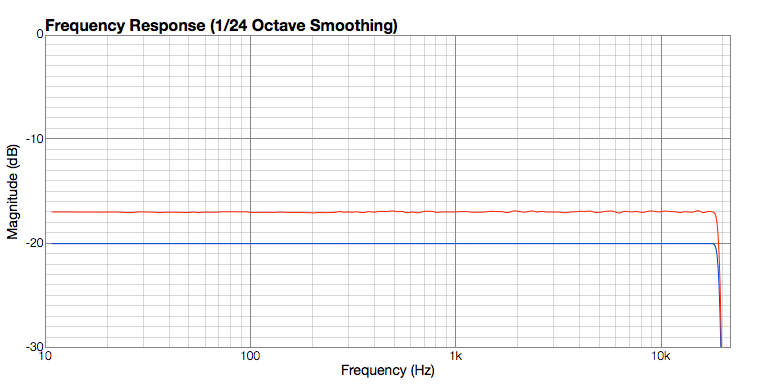
\includegraphics[height=0.3\textwidth]{figures/surround.png}
\end{figure}

\end{frame}
